\documentclass[fleqn]{article}
\oddsidemargin 0.0in
\textwidth 6.0in
\thispagestyle{empty}
\usepackage{import}
\usepackage{amsmath}
\usepackage{graphicx}
\usepackage{flexisym}
\usepackage{amssymb}
\usepackage{bigints} 
\usepackage[english]{babel}
\usepackage[utf8x]{inputenc}
\usepackage{float}
\usepackage[colorinlistoftodos]{todonotes}

\definecolor{hwColor}{HTML}{AD53BA}

\begin{document}

  \begin{titlepage}

    \newcommand{\HRule}{\rule{\linewidth}{0.5mm}} % Defines a new command for the horizontal lines, change thickness here

    \center % Center everything on the page



    \textsc{\LARGE Arizona State University}\\[1.5cm] % Name of your university/college

    \textsc{\LARGE Mathematical Methods For Physics II }\\[1.5cm] % Major heading such as course name


    \begin{figure}
      
\includegraphics[width=\linewidth]{asu.png}
    \end{figure}


    \HRule \\[0.4cm]
    { \huge \bfseries Homework Eleven}\\[0.4cm] 
    \HRule \\[1.5cm]

    \textbf{Behnam Amiri}

    \bigbreak

    \textbf{Prof: Cecilia Lunardini}

    \bigbreak


    \textbf{{\large \today}\\[2cm]}

    \vfill % Fill the rest of the page with whitespace

  \end{titlepage}

  \textbf{Part A}
  \begin{enumerate}

    \item Prove the \emph{completeness relationship}, eq. (18.51) of the textbook. (Hint: treat the Dirac Delta like you would treat a generic function, and write it in the basis of the Spherical Harmonics). 
    
      \textcolor{hwColor}{
        \\
        We need to write down the equation $(18.51)$ from the textbook.
        $$\sum\limits_{n=0} Y^m_{\ell}(\Omega) ~ Y^{m*}_{\ell}(\Omega^')=\delta(\Omega-\Omega^')$$
        From page 594 of the textbook we have \begin{itemize}
          \item $\delta(\Omega-\Omega^')=0$ if $\Omega$
          \item $\bigints_{4 \pi} \delta(\Omega) d\Omega=1$
        \end{itemize}
        Since we are told, we can treat the Dirac Delta like we would treat a generic function in the he S.H. ,
        then let's treat it as an arbitrary function. Then we plug in the dirac to get the closure relationship.\\
        \\
        $
          f(\Omega)=\delta(\Omega-\Omega^') \equiv \delta(cos(\theta)-cos(\theta^'))\delta(\phi-\phi^') \\
          \\
          \\
          \therefore ~~~ \delta(\Omega-\Omega^')=\bigints\limits_{4 \pi} f(\Omega^') \sum\limits_{\ell m} Y^m_{\ell}(\Omega^') Y^m_{\ell}(\Omega) d\Omega^' \\
          \\
          \\
          \therefore ~~~ =\bigints\limits_{4 \pi} \delta(cos(\theta)-cos(\theta^')) \delta(\phi-\phi^') \sum\limits_{\ell m} Y^m_{\ell}(\Omega^') Y^m_{\ell}(\Omega) d\phi ~ d(cos(\theta)) \\
          \\
          \\
          \therefore ~~~ =\sum\limits_{\ell m} Y^m_{\ell}(\Omega^') Y^m_{\ell}(\Omega) \times \bigints\limits_{4 \pi} \delta(cos(\theta)-cos(\theta^')) \delta(\phi-\phi^') d\phi ~ d(cos(\theta))
        $
        \\
        \\
        The above integral equals to one, hence we have: \\
        \\
        \\
        $
          \therefore ~~~ \sum\limits_{\ell m} Y^m_{\ell}(\Omega^') Y^m_{\ell}(\Omega) \times 1
          \\
          \\
          \\
          \therefore \delta(\Omega-\Omega^')=\sum\limits_{\ell m} Y^m_{\ell}(\Omega^') Y^m_{\ell}(\Omega) ~~~ \surd
        $ 
      }
    
    \item Prove that the differential equation that has $\sin( k x)$ and $\cos(k x)$ as solutions (with $k$ a constant) is a Sturm-Liouville equation. 
    
      \textcolor{hwColor}{
        The general form of the Sturm-Liouville equation is (page 564)
        $$p(x) \dfrac{d^2 y}{dx^2}+r(x) \dfrac{dy}{dx}+q(x)y+\lambda \rho(x) y=0, ~~~~~ r(x)=\dfrac{dp(x)}{dx}, ~~~~ \mathbf{(A)}$$
        \\
        \\
        For a simple harmonic $\dfrac{d^2y}{dx}+k^2 y=0, ~ \mathbf{(B)}$, we know that the general solution is 
        $$y(x)=A ~ sin(kx)+B ~ cos(kx)$$ \\
        By equating $\mathbf{(A)}$ and $\mathbf{(B)}$ we get the following result: \\
        \\
        $
          \begin{cases}
            p(x)=1 \\
            \rho(x)=1 \\
            q(x)=0 \\
            \lambda=k^2
          \end{cases}
        $
        \\
        \\
        Using the condition that $r(x)=p^'(x)$ it will be seen that the general Sturm-Liouville equation can also
        be rewritten as $\left(p \dfrac{dy}{dx}\right)^'+qy+\lambda \rho y=0$.  
        \\
        \\
        By plugging the above values into equation $(17.34)$ we have: \\
        \\
        \\
        $
          \left(1 \times \dfrac{dy}{dx}\right)^'+\left(0 \times y\right)+\left(k^2 \times 1 \times y\right)=0 \\
          \\
          \\
          \therefore ~~~~ \dfrac{d^2}{dx^2}+k^2 y=0 ~~~ \surd
        $
        \\
        \\
        The O.D.E that we just presented is a demonstration of the Sturm-Liouville differential equation.  
      }
    
    \item Consider a system of three point-like electric charges, with charges $q_i$ and positions $\vec r_i$ ($i=1,2,3$), as follows:
    $q_1=+Q$, $\vec r_1=(0,0,d)$; $q_2=+Q$, $\vec r_2=(d,0,0)$; $q_3=-Q$, $\vec r_3=(0,0,0)$.   
    
    \begin{enumerate}
      \item Calculate the ``outer" monopole moment of the given system of charges. 
      
      \item Calculate the ``outer" dipole moment for $m=0$. 
    
    \end{enumerate}
    (Hint: follow the example shown in class). 

    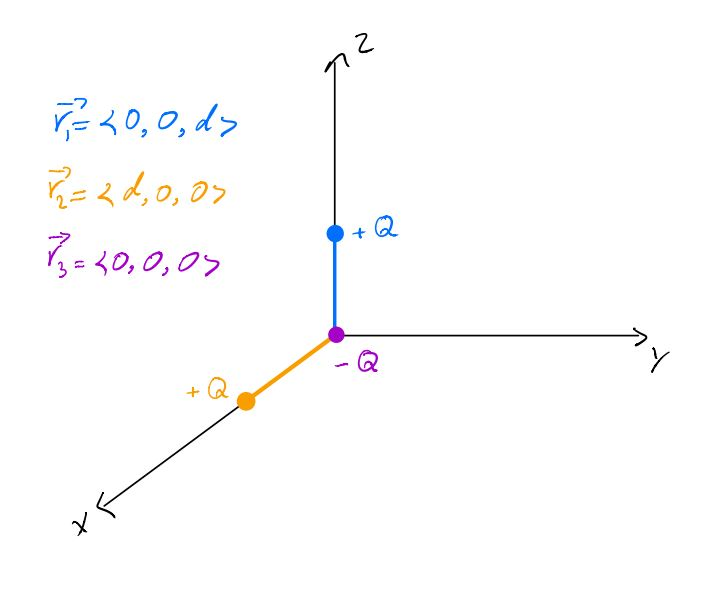
\includegraphics[height=10cm, width=12cm]{One.JPG}

      \textcolor{hwColor}{
        Let's start off with the multipole moment equation 
        $$p^m_n=\bigints r^n_s \rho_Q(\overrightarrow{r_s}) Y^{m*}_n \left(\hat{r_s}\right) d^3 \overrightarrow{r_s}$$ \\
        \\
        \\
        \begin{itemize}
          \item $r_s$ refers to the magnitude of the vector pointing from the origin to the each piece of the source of the
          electric potential in question. 
          \item $\rho_Q(\overrightarrow{r_s})$ is the charge density of the source.
          \item $Y^{m*}_n \left(\hat{r_s}\right)$ is the complex conjugate of a spherical harmonic. 
        \end{itemize}
      }

      \textcolor{hwColor}{
        \\
        \\
        $
          \rho_Q(\overrightarrow{r_s})=Q \delta(x) \delta(y) \delta(z)+Q \delta(x+d) \delta(y) \delta(z)+Q \delta(x) \delta(y) \delta(z)
        $
        \\
        \\
        We want to use the three dimensional direct delta written in spherical polar form. 
        Referencing Theory Segment 16, the spherical polar form of the
        three-dimensional Dirac delta is 
        \\
        \\
        $
          \delta^3(\mathbf{r}-\mathbf{r_0})=\dfrac{1}{r^2_0} \delta(r-r_0) \delta(cos\theta-cos \theta_0) \delta(\phi-\phi_0)
        $
        \\
        \\
        Let's have the spherical polar coordinate of those three given points. \\
        \\
        $
          \begin{cases}
            r_1=<d,0,\phi_0> \\
            \\
            r_2=<d, \dfrac{\pi}{2}, 0> \\
            \\
            r_3=<0,0,0>
          \end{cases} \\
          \\
          \\
          \\
          \rho_Q(\overrightarrow{r_s})= \\
          Q \dfrac{1}{r^2_s} \delta(r_s-d) \delta(cos(\theta)-1) \delta(\phi-\phi_0) \\
          +Q \dfrac{1}{r^2_s} \delta(r_s-d) \delta(cos(\theta)) \delta(\phi-\phi_0) \\
          +Q \dfrac{1}{r^2_s} \delta(r_s) \delta(cos(\theta)-1) \delta(\phi-\phi_0) \\
          \\
          \\
          \\
          \therefore ~~~ \rho_Q(\overrightarrow{r_s})=Q \dfrac{1}{r^2_s} \delta(\phi-\phi_0) \left[
            \delta(r_s-d) \delta(cos(\theta)-1) 
            +\delta(r_s-d) \delta(cos(\theta)) 
            + \delta(r_s) \delta(cos(\theta)-1)
          \right] ~~~~ \surd
          \\
          \\
          \\
        $
        The infinitesimal volume element, $d^3\overrightarrow{r_s}$ in spherical polar coordinates is: \\
        \\
        $
          d^3\overrightarrow{r_s}=r^2_s dr_s sin(\theta)d\theta d\phi=r^2_s dr_s d(cos(\theta)) d\phi
        $
        \\
        \\
        Now, let’s plug in our volume element and our expression for $\rho_Q(\overrightarrow{r_s})$
        into the equation for the multipole moments. \\
        \\
        \\
        $
          p^m_n=\bigints r^n_s \rho_Q(\overrightarrow{r_s}) Y^{m*}_n(\theta, \phi) \left(\hat{r_s}\right) d^3 \overrightarrow{r_s} \\
          \\
          \\
          =\bigints r^n_s Q \dfrac{1}{r^2_s} \delta(\phi-\phi_0) \left[
            \delta(r_s-d) \delta(cos(\theta)-1) 
            +\delta(r_s-d) \delta(cos(\theta)) 
            + \delta(r_s) \delta(cos(\theta)-1)
          \right] Y^{m*}_n(\theta, \phi) \left(\hat{r_s}\right) r^2_s dr_s d(cos(\theta)) d\phi \\
          \\
          \\
          \\
          =Q r^n_s \bigints Y^{m*}_n(\theta, \phi) \delta(\phi-\phi_0) \left[
            \delta(r_s-d) \delta(cos(\theta)-1) 
            +\delta(r_s-d) \delta(cos(\theta)) 
            + \delta(r_s) \delta(cos(\theta)-1)
          \right] d(cos(\theta)) d\phi
        $
        \\
        \\
        Now, because we took $\phi_0$ to be arbitrary, \emph{any} choice of this angle must give
        us the same result for $p^m_n$. In other words, the multipole moments must
        be independent of $\phi_0$. However, we also know that the spherical harmonics
        have non-trivial $\phi$ behavior, with the exception of the spherical harmonics for
        which $m=0$. Next, since $\phi$ is completely arbitrary, we will choose $\phi_0=0$.
        \\
        \\
        Substituting $m=0$ and $\phi_0=0$ and evaluating the integral: \\
        \\
        \\
        $
          p^m_n=Q d^n \bigints Y^{m*}_n(\theta, \phi) \delta(\phi-\phi_0) \left[
            \delta(r_s-d) \delta(cos(\theta)-1) 
            +\delta(r_s-d) \delta(cos(\theta)) 
            + \delta(r_s) \delta(cos(\theta)-1)
          \right] d(cos(\theta)) d\phi
        $
      }
    
  \end{enumerate}

  \textbf{Part B}
  \begin{enumerate}

    \item Using the definition of analytic function, determine which of the complex functions below are analytic: 
    
      \textcolor{hwColor}{
        \\
        From lecture and from page 826 of the textbook, we saw that we defined a function as analytic 
        if it was single-valued and differentiable at all points in a domain $\mathcal{R}$ where we defined differentiability 
        as the unique existence of the following expression (equation 24.1 in the textbook): \\
        \\
        $$f(z)=\lim\limits_{\Delta z \to 0} \left[\dfrac{f(z+\Delta z)-f(z)}{\Delta z}\right]$$
      }
    
    \begin{enumerate}
      \item $F(x,y)=x^2+2ixy+y^2$;

        \textcolor{hwColor}{
          $
            F^'(x,y)=\lim\limits_{\Delta x,\Delta y  \to 0} \left[\dfrac{F(x+\Delta x,y+\Delta y)-F(x,y)}{\Delta x+i \Delta y}\right] \\
            \\
            \\
            =\lim\limits_{\Delta x,\Delta y  \to 0} \left[\dfrac{ (x+ \Delta x)^2+2i(x+\Delta x)(y+\Delta y)+(y+\Delta y)^2- \left(x^2+2ixy+y^2\right)}{\Delta x+i \Delta y}\right] \\
            \\
            \\
            =\lim\limits_{\Delta x,\Delta y  \to 0} \left[\dfrac{2\left(x \Delta x+y \Delta y\right)+\Delta x^2+\Delta y^2 +2i \left(y \Delta x+x \Delta y+\Delta x \Delta y \right)}{\Delta x+i \Delta y}\right]
          $ \\
          \\
          \\
          At this point, we are stuck - no matter what we do, we will not be able to get rid of the terms involving $\dfrac{\Delta y}{\Delta x}$, hence it is not analytic. \\ \\ \\
        }

      \item $F(x,y)=x^2-y^2$;

        \textcolor{hwColor}{
          $
            F^'(x,y)=\lim\limits_{\Delta x,\Delta y  \to 0} \left[\dfrac{F(x+\Delta x,y+\Delta y)-F(x,y)}{\Delta x+i \Delta y}\right] \\
            \\
            \\
            =\lim\limits_{\Delta x,\Delta y  \to 0} \left[\dfrac{ (x- \Delta x)^2-(y+\Delta y)^2 -x^2+y^2}{\Delta x+i \Delta y}\right] \\
            \\
            \\
            =\lim\limits_{\Delta x,\Delta y  \to 0} \left[\dfrac{2(x\Delta x - y\Delta y)+ \Delta x^2 -\Delta y^2 }{\Delta x+i \Delta y}\right] \\
            \\
            \\
          $
          At this point, we are stuck - no matter what we do, we will not be able to get rid of the terms involving $\dfrac{\Delta y}{\Delta x}$, hence it is not analytic. \\ \\ \\
        }

      \item $F(x,y)=x^2-2ixy-y^2$;

        \textcolor{hwColor}{
          $
            F^'(x,y)=\lim\limits_{\Delta x,\Delta y  \to 0} \left[\dfrac{F(x+\Delta x,y+\Delta y)-F(x,y)}{\Delta x+i \Delta y}\right] \\
            \\
            \\
            =\lim\limits_{\Delta x,\Delta y  \to 0} \left[\dfrac{(x+\Delta x)^2-2i(x+\Delta x)(y+\Delta y)-(y+\Delta y)^2-x^2+2ixy+y^2}{\Delta x+i \Delta y}\right] \\
            \\
            \\
            =\lim\limits_{\Delta x,\Delta y  \to 0} \left[\dfrac{\Delta x^2+2x \Delta x-\Delta y^2-2y \Delta y-2i(y \Delta x+x \Delta y+\Delta x \Delta y)   }{\Delta x+i \Delta y}\right] \\
            \\
            \\
            =\lim\limits_{\Delta x,\Delta y  \to 0} \left[\dfrac{(\Delta x-i \Delta y)\left(\Delta x+2x-i(\Delta y+2y)\right)}{\Delta x+i \Delta y}\right] \\
            \\
            \\
          $
          At this point, we are stuck - no matter what we do, we will not be able to get rid of the terms involving $\dfrac{\Delta y}{\Delta x}$, hence it is not analytic. \\ \\ \\
        }
  
      \item $F(x,y)=x^2+2ixy-y^2$;

        \textcolor{hwColor}{
          $
            F^'(x,y)=\lim\limits_{\Delta x,\Delta y  \to 0} \left[\dfrac{F(x+\Delta x,y+\Delta y)-F(x,y)}{\Delta x+i \Delta y}\right] \\
            \\
            =\lim\limits_{\Delta x,\Delta y  \to 0} \left[\dfrac{(x+\Delta x)^2+2i(x+\Delta x)(y+ \Delta y)-(y+\Delta y)^2-x^2-2ixy+y^2}{\Delta x+i \Delta y}\right] \\
            \\
            \\
            =\lim\limits_{\Delta x,\Delta y  \to 0} \left[\dfrac{2(x+iy)(\Delta x+i \Delta y)-(\Delta x+i \Delta y)^2}{\Delta x+i \Delta y}\right] \\
            \\
            \therefore ~~~~ F^'(x,y)=2(x+iy) ~~~~ \surd \\ \\
          $
          Hence it is analytic.
        }

      \item $F(x,y)=e^x(\cos y+i \sin y)$;

        \textcolor{hwColor}{
          $
            F(x,y)=e^x(\cos y+i \sin y)=e^x e^{iy} \\ \\
            \therefore ~~~ F(x,y)=e^z \\ \\
            F^'(x,y)=\lim\limits_{\Delta z  \to 0} \left[\dfrac{F(z+\Delta z)-F(z)}{\Delta z}\right] \\
            \\
            \\
            =\lim\limits_{\Delta z  \to 0} \left[\dfrac{e^{z+ \Delta z}-e^z}{\Delta z}\right] \\
            \\
            \\
            =\lim\limits_{\Delta z  \to 0} \left[e^z \left(\dfrac{e^{\Delta z}-1}{\Delta z}\right)\right] ~~~~ (\mathbf{H})\\
            \\
            \\
            =e^z \lim\limits_{\Delta z  \to 0} e^{\Delta z} \\
            \\
            \\
            \therefore ~~~  F^'(x,y)=e^z ~~~ \surd \\ \\
          $
          Hence it is analytic. \\ \\ \\ 
        }

      \item $F(x,y)=e^y(\cos x+i \sin x)$.

        \textcolor{hwColor}{
          $
            F(x,y)=e^y(\cos x+i \sin x)=e^y e^{ix}=e^{y+ix} \\ \\
            F^'(x,y)=\lim\limits_{\Delta x,\Delta y  \to 0} \left[\dfrac{F(x+\Delta x,y+\Delta y)-F(x,y)}{\Delta x+i \Delta y}\right] \\
            \\
            \\
            =\lim\limits_{\Delta x,\Delta y  \to 0} \left[\dfrac{e^{(y+\Delta y)+i(x+\Delta x)} -e^{y+ix}}{\Delta x+i \Delta y}\right] \\
            \\
            \\
            =\lim\limits_{\Delta x,\Delta y  \to 0} \left[\dfrac{e^{\Delta y+i \Delta x}}{\Delta x+i \Delta y}\right]
          $
          \\
          \\
          At this point, we are stuck - no matter what we do, we will not be able to get rid of the terms involving $\dfrac{\Delta y}{\Delta x}$, hence it is not analytic. \\ \\ \\
        }

    \end{enumerate}
    
    \item Apply the Cauchy Riemann conditions to the complex functions in the Exercise 1 above.
    
    \textcolor{hwColor}{
      Another method of determining whether a function is analytic involves 
      applying the Cauchy-Riemann conditions, given by equation 24.5 in the textbook.
      $$\begin{cases}
        \dfrac{\partial u}{\partial x}=\dfrac{\partial v}{\partial y} \\
        \\
        \dfrac{\partial v}{\partial x}=-\dfrac{\partial u}{\partial y}
      \end{cases}$$
      \\
      \\
      where the functions $u(x, y)$ and $v(x, y)$ are obtained from $f(z)$ by rewriting it as 
      $f(z) =u(x, y) +iv(x, y)$. If each of these partial derivatives is continuous in the domain
      in question, and if these two relations are satisfied, the functionis analytic. \\
      \\
      $
        F(x,y)=x^2+2ixy+y^2 \\
        \\
        u=x^2+y^2, ~~ v=2xy \\
        \\
        \begin{cases}
          \dfrac{\partial u}{\partial x}=\dfrac{\partial v}{\partial y}=2x \\
          \\
          \dfrac{\partial v}{\partial x}=2y \\
          \\
          -\dfrac{\partial u}{\partial y}=-2y
        \end{cases}
      $
      Hence, it is not analytic. 
      \\
      \\
      \rule{15cm}{1pt}
      \\
      \\
      $
        F(x,y)=x^2-y^2
      $
      \\
      \\
      \rule{15cm}{1pt}
      \\
      \\
      $
        F(x,y)=x^2-2ixy-y^2
      $
      \\
      \\
      \rule{15cm}{1pt}
      \\
      \\
      $
        F(x,y)=x^2+2ixy-y^2
      $
      \\
      \\
      \rule{15cm}{1pt}
      \\
      \\
      $
        F(x,y)=e^x(\cos y+i \sin y)
      $
      \\
      \\
      \rule{15cm}{1pt}
      \\
      \\
      $
        F(x,y)=e^y(\cos x+i \sin x)
      $
    }
    
  \end{enumerate}

\end{document}
